%!TEX root = ../../dissertacao.tex
\label{chap:inductive}
This chapter brings a brief introduction on formal verification and a more detailed explanation on the selected approach to be used in this work: the Inductive Method. Its syntax will be restrained for comprehension of the proposed problem.

\section{Formal Verification}
Using the previous definitions for security protocols, it is easy to perceive that one can reason about protocol rules, \textit{verifying} if they are correct with respect to the protocol's goals.

Informal reasoning on verifying protocols was the first attempt to guarantee their correctness, succeeding in recognizing some flaws and weaknesses quickly and providing a good understanding about protocols designs \cite{bella-book}. However, not finding an error does not mean that a certain model does not hold one. Such method was failing to identify critical flaws in major security protocols, where the classical example of the Needham-Schroeder protocol \cite{needham-schroeder} can be cited. The techniques in \cite{lowe96} exposed the protocol's limitations, despite the authors efforts on its specification and informal verification.

This scenario was optimal for the rise of formal verification on security protocols such as in the works presented in \cite{meadows-old-survey}, \cite{kemmerer-verification} and \cite{ban}, allowing a mathematical and profitable procedure for reasoning about abstract protocols models. Thus, it is important to emphasize that the method focus on the protocol properties and rules, and rarely on its execution.

Formal verification requires the definition of such protocols in a proper language, suitable for the application of such methods and deservedly automated through computational methods. Formal methods can be divided in two major categories, according to \cite{boyd-mathuria}:

\begin{itemize}
  \item \textbf{Model checking}: protocol behaviors can be modeled as a finite set of states. Such proposal is suitable for checking if a given configuration satisfy a set of correctness conditions and analyze a certain past configuration, searching for attacks attempts. This approach is more appropriate for finding inconsistencies and attacks in the protocol rather than proving its correctness;

  \item \textbf{Theorem proving}: postulating the protocol as a theorem, taking into account \textit{all} possible protocol behaviors, and checking its correctness through the verification of the theorem claims. This method is more suitable for proving the correctness of the protocol rather than finding possible attacks on them.
\end{itemize}

Both methods are aided by computer assistance, where theorem proving may be a less automated approach. Concerning the protocol analyzed in this document and our goal to prove its correctness, it is trivial to guess that our chosen method fits the theorem proving set.

\section{Method Introduction}
Induction has been a commonly used mathematical proof method among theorem proving literature. Proving inductively a certain property $P(n)$ demands a base case $P(0)$ and the validation of general formula $P(i) \Rightarrow P(i + 1)$, for all $i > 0$, concluding that $P(n)$ is true, for any positive integer $n$. It is reasonable to apply this procedure on security protocols, where one can check if a security property is preserved along a large population of participants and all possible system executions. The work of L.~Paulson \cite{paulson-inductive} was the first to propose such idea and it has been extended by G.~Bella in \cite{bella-book}.

The model considers a protocol $\mathcal{P}$ and an unlimited set of agents, which includes the Spy, an omnipotent entity. Agents actions result in network traffic, which is abstracted as a \textbf{trace}: a history of events in the network, displayed in reversed chronological order. Therefore, we can define the set $P$, containing all possible traces of infinite length as a formal model of the environment where the protocol ran. Such set is defined inductively by the rules of $\mathcal{P}$.

This approach has much in common with CSP formalizations \cite{ryan-schneider}, although the traces considered here are infinite. Besides, the method only focus on security properties, not considering liveness (denial of service), for example.

\subsection{Isabelle}
One of the most interesting characteristics of the Inductive Method is the possibility of proof mechanization by means of the theorem prover Isabelle \cite{isabelle}. The generated proofs are machine checkable, enabling a deep understanding of its anatomy and easy error maintenance.

Isabelle is a generic theorem prover, meaning that it is able to reason over several formal systems, in an interactive way: its not entirely automatic, requiring certain human interaction for concluding proofs. At the same time, it offers automatic provers, which can deal with several simple proofs, and it also provides simplifiers methods, enabling rewriting of expressions with adequate arithmetic procedures.

The version in which this document is based is Isabelle/HOL \cite{isabelle-hol}, based on high-order logics. This kind of logics can quantify over functions, predicates and sets, based on a strongly typed formalism. Moreover, most of the proofs may be produced inductively, where often subgoals are left for being simplified. In case any subgoals are left unsimplified, the user must provide lemmas for complementing the rewriting rules and finally proving the main theorem.

Due to that, some proofs may take time and patience. If a user fail to find a proof for a certain property, this may not be a certification of proof unsatisfiability. Despite, the proof or somes of its aspects may be built on top of wrong formalizations, meaning the user is not skilled enough.

Along this chapter, Isabelle syntax on security protocol properties will be presented. Basic operations and symbols will be explained when convenient, but aiming document readability, most part of the syntax will be omitted. An extensive and reliable literature on theorem proving on Isabelle is available in \cite{isabelle-hol} and security protocol proofs in \cite{bella-book}.



\section{Formalizing Entities}
For a suitable verification of the system, a prior definition of it is necessary. In the context of Isabelle, a theory is such specification, containing a set of definitions and theorems which need to be proven for a solid formalization. Isabelle has a large collection of theories, within many areas, including the one concerning this work \cite{isabelle-hol-auth}.

The \texttt{Auth} library from Isabelle/HOL distribution \cite{isabelle-hol-auth} provides a set of theories, which consist of sets of definitions and theorems for reasoning about security protocols, enabling a researcher to build proofs with solid base and quick setup. Here, we introduce such concepts, which are essential for understanding the inductive way to work with formal verification of security protocols.

\subsection{Agents}
This is the basic type for defining participants in a protocol session. The model considers an infinite set, due to the possible large population of active peers. A simple bijection with the set of natural numbers can shape the main principals of a protocol: Friend, Spy and Server. Such entities can be compactly defined in Isabelle syntax as follows:

\begin{center}
  $\texttt{datatype agent} \triangleq \texttt{Server } | \texttt{ Spy } | \texttt{  Friend nat}$
\end{center}

The \texttt{Friend} definition is the common peer in a session. Since we can have a positive infinite number of participants, we simply define the $i$-th peer as \texttt{Friend $i$}. The entity \texttt{Spy} is used as a formal representation of a threat model (which will be defined later), defined with a nullary constructor. Finally, the \texttt{Server} entity, often represented as \texttt{S}, is a commonly trusted third-party agent, used for symmetric key generation operations. Additionally, this peer has access to all agents long-term secrets, i.e., the private keys of other agents or servers.

Thus, a characterization of compromised agents is made. These are embedded in an unspecified set named \texttt{bad}, where the Spy is also included. All elements within this set have their knowledge set exposed to the Spy, which includes private keys, shared keys with the Server and any other secrets. This property takes action along all protocol run, which means that if the agent notes any information during a session, the Spy is able to retrieve it.

\subsection{Cryptographic Keys}
Keys are the base entity for providing encryption and they have several groups. Here, they are declared as a free type, but interpreted as an integer and each kind of key has intrinsic properties, as follows.

For cryptographic symmetric keys, exchanged with trusted servers - the \texttt{Server} entity - the key is previously stored by an agent. So, it is defined as a agent dependent value:

\begin{center}
  \texttt{shrK : agent} $\rightarrow$ \texttt{key}
\end{center}

This declaration is also applicable for asymmetric keys, where the notation is \texttt{priK} for private one and \texttt{pubK} for the public. This notation may differ when a signature key is used.

Symmetric keys are a bigger scope for other keys, belonging to a proper set \texttt{symKeys}. One example are session keys, which are used by peers for establishing a single private session of communication. Therefore, the valid definition is:

\begin{center}
  $K \in \texttt{symKeys} \text{ and } K \notin \texttt{range shrK}$
\end{center}

Such definition implies that the set of shared keys is different from the one containing session keys. Any other kind of keys not mentioned here must be manually defined.

\subsection{Messages}
A message is any kind of information that can be transmitted during the execution of a protocol. This includes agents names, keys, nonces, timestamps, and so on. Therefore, the constructor of a \texttt{Message} variable accepts many kinds of formats, as stated below:

\begin{equation*}
  \begin{split}
    \texttt{datatype} \triangleq
    & \texttt{\textbf{Agent} agent} \\
    & \texttt{\textbf{Nonce} nat} \\
    & \texttt{\textbf{Key} key} \\
    & \texttt{\textbf{Mpair} msg msg} \\
    & \texttt{\textbf{Hash} msg} \\
    & \texttt{\textbf{Crypt} key msg}
  \end{split}
\end{equation*}

Some of the accepted datatypes are constructors and others are simply natural numbers. If any other datatype is needed, the definition of this scope must be extended. It is important to notice that the \texttt{Mpair} constructor enables the definition of recursive concatenation of messages.

Another important concept is the \texttt{Crypt} directive. This is used for representing encryption of messages, such as message $M$, with key $K$, denoted by \texttt{Crypt K M}. In this model, encryption is perfect and collision-free, so the $M$ is only accessible if the peer have the key $K$.

\subsection{Events}
Events are a basic entity along protocols. Here we present the definition of the three main kinds of events, suitable for the analyzed protocol in this work, although there are more available for others protocols:

\begin{equation*}
  \begin{split}
    \texttt{datatype} \triangleq
    & \texttt{\textbf{Says} agent agent msg} \\
    & \texttt{\textbf{Notes} agent msg} \\
    & \texttt{\textbf{Gets} agent msg}
  \end{split}
\end{equation*}

The action of \texttt{Says} is straightforward and it follows easily from its syntax: the first agent is the sender, the second is the intended receiver and the third parameter is the message which will be sent.

However, it is necessary to settle the difference between \texttt{Notes} and \texttt{Gets}. The former relates to the action of noting down fragments of data from received messages, which is particularly used by the Spy for deriving keys sent in inaccurate peers messages. The latter is technically equivalent to the \texttt{Notes} action. At the same time, it does not implies the storage of an information, not enriching the set of known entities of an agent or of a given trace. This leaves the definitions and rule construction leaner.

Now, the definition of a \textbf{trace} can be done. Intending to keep an history of the network, a trace is a list of events that occur in the network, displayed in reverse chronological order. Therefore, every single event that occurred in the network while the protocol was active must be present in the trace. Besides, the trace must respect the protocol model, since it can only be constructed upon a valid run of the given protocol.

\subsection{Nonces, Timestamps and Guessable Numbers}
Security protocols often resort on numeric entities for soundness of some properties. These numbers are modeled as well, but they come with premises for being compatible with reality.

\textbf{Nonces} are random numbers, hence they are modeled this way. In the Inductive Method, they are shaped as a big random natural number and are unguessable. Additionally, they are designed to provide freshness and, consequently, are supposed to be out of the set which contains all messages that are clear in the network. This set, named \texttt{used}, will be defined in a latter section.

\textbf{Guessable numbers} are the opposite. Intuitively, they are considered natural numbers, but they are guessable. As a result, they are always known by the Spy. Thus, the message datatype is extended to cover this primitive, with the declaration \texttt{Number N}.

\textbf{Timestamps} relies in the notion of time in protocols. Such concept is provided when each event of a trace carries the time instant when it happened, so it is straightforward to define a valid time model for the local trace. The authors note that the temporal relations are irrelevant between traces, since they are different runs of protocols. Also, this representation excludes the concept of concurrency: two events can never happen simultaneously in a trace. It is argued that this notion of concurrency can be represented when two events are sequentially interleaved in two different traces. Finally, the definition of current time is done:

\begin{center}
  \texttt{CT evs} $\triangleq$ \texttt{length evs}
\end{center}

This definition makes sense, since the time of the last event dictates the current time on the trace. Such definition need the function below:

\begin{center}
  \texttt{CT : event list} $\longrightarrow$ \texttt{nat}
\end{center}


\subsection{Operators}
In the Inductive Method, the actions of reasoning about and composing messages are treated as operations over sets of messages. In that way, the operators \texttt{analz}, \texttt{synth} and \texttt{parts} are defined upon operations on this kind of data:

\begin{center}
  \texttt{analz, synth, parts : msg set $\longrightarrow$ msg set}
\end{center}

The \texttt{analz} operator denotes the act of inspecting the components of a message and then breaking it up. Therefore, using the set of messages $H$, the set \texttt{analz} $H$ uses the following rules:

\begin{enumerate}
  \item Any element of a message set $H$ can be analyzed from it;
  \begin{center}
    $X \in H \Longrightarrow X \in$ \texttt{analz} $H$
  \end{center}

  \item Any element in a given concatenation of messages, that could be analyzed from its message set, can also be analyzed from it;
  \begin{center}
    $\Bracks{X,Y} \in \texttt{analz} H \Longrightarrow X \in$ \texttt{analz} $H$ \\
    $\Bracks{X,Y} \in \texttt{analz} H \Longrightarrow Y \in$ \texttt{analz} $H$
  \end{center}

  \item The contents of an analyzed ciphertext can only properly be analyzed and further retrieved in possession of its decryption key.
  \begin{center}
    $\lBrace$\texttt{Crypt} $K$ $X$ $\in$ \texttt{analz} $H$; \texttt{Key(invKey} $K$\texttt{)} $\in$ \texttt{analz} $H\rBrace$ $\Longrightarrow$ $X$ $\in$ \texttt{analz} $H$
  \end{center}
\end{enumerate}

It is significant to mention the set \texttt{analz(spies) \textit{evs}}. This set holds all data that the Spy could gather from the network in the trace \textit{evs}, either by decomposing it from another messages or obtaining from decrypted ciphertexts, defining its current knowledge set. Thus, saying a set of message $X$ does not belong to this set is equivalent to state the confidentiality of $X$ in such trace.

The second operator is the \texttt{synth}, which basically denotes the action of composing messages from given components. Its rules are the following:

\begin{enumerate}
  \item Any element or agent name can be synthesized from a message set;
  \begin{center}
    $X \in H \Longrightarrow X \in$ \texttt{synth} $H$ \\
    \texttt{Agent} $A \in$ \texttt{synth} $H$
  \end{center}

  \item If a message can be synthesized from a message set, then so it can its hash;
  \begin{center}
    $X \in$ \texttt{synth} $H \Longrightarrow$ Hash $X \in$ \texttt{synth} $H$
  \end{center}

  \item If two messages can be synthesized from a message set, then so it can its concatenation;
  \begin{center}
    $\Braces{X \in \texttt{synth } H; Y \in \texttt{synth } H} \Longrightarrow \Bracks{X,Y} \in$ \texttt{synth} $H$
  \end{center}

  \item If a key belongs to a message set and a message can be synthesized from it as well, then so the encryption of the message with the given key.
  \begin{center}
    $\Braces{\texttt{Key } K \in H; X \in \texttt{synth } H} \Longrightarrow$ \texttt{Crypt} $K X \in$ \texttt{synth} $H$
  \end{center}
\end{enumerate}

Finally, the last operator \texttt{parts} is very similar to the \texttt{analz} operator, hence its rules are similar to the latter, except the one concerning encryption. In this operator, the extraction of a ciphertext from a encrypted message does not require a key. Thus, we can relate both operators in such way: \texttt{analz} $\subseteq$ \texttt{parts}. Such concept simulates unbounded computational power and so, the rule is rewritten as follows:

\begin{center}
  $\texttt{Crypt } K X \in \texttt{parts } H \Longrightarrow X \in$ \texttt{parts} $H$
\end{center}

Complementing the crucial sets for the method, it is introduced the set \texttt{used}, which is used to delimit the set of already used message components, belonging to some agent initial knowledge or which have appeared at some moment in the network. Such concept is important due to the necessity of working with the freshness concept and properly modeling it. The definition of the set follows:

\begin{center}
  \texttt{used : event list} $\longrightarrow$ \texttt{msg set}
\end{center}

\subsection{Initial Assumptions}
\label{sec:initial-assumptions}
In order to be compatible with real world context, the Inductive Method provide some basic initial definitions concerning several aspects of the environment and principals.

First, a formalization of agents initial knowledge set is provided. Such definition is important not only for stating the protocol initial premises, but for constructing the initial knowledge of the attacker, based in the compromised agents. Thereby, we define the function \texttt{initState}, which receives an agent as argument and returns the agent's initial knowledge message set:

\begin{center}
  \texttt{initState : agent} $\longrightarrow$ \texttt{msg set}
\end{center}

For every different kind of agent, we have a different type of initial knowledge set:

\begin{enumerate}
  \item The Server initially knows all shared and public keys and its own private keys;

  \begin{equation*}
    \begin{split}
      \texttt{initState Server} \triangleq
      & (\texttt{Key range shrK}) \  \cup \\
      & \{\texttt{Key (priEK Server)}\} \cup \{\texttt{Key (priSK Server)}\}\  \cup \\
      & \texttt{(Key range pubEK)} \cup \texttt{(Key range pubSK)}
    \end{split}
  \end{equation*}


  \item Each legitimate agent (\texttt{Friend}) initially knows its own shared and private keys and all public keys;

  \begin{equation*}
    \begin{split}
      \texttt{initState (Friend \textit{i})} \triangleq
      & \{ \texttt{Key (shrK (Friend \textit{i}))} \} \ \cup \\
      & \{ \texttt{Key (priEK (Friend \textit{i}))} \} \ \cup \\
      & \{ \texttt{Key (priSK (Friend \textit{i}))} \} \ \cup \\
      & \texttt{(Key range pubEK)} \cup \texttt{(Key range pubSK)}
    \end{split}
  \end{equation*}


  \item The Spy knows all secrets from the agents who belong to the compromised set, which includes shared and private keys, including herself, since she is included in the set of compromised peers. Additionally, she also knows all public keys.

  \begin{equation*}
    \begin{split}
      \texttt{initState Spy} \triangleq
      & (\texttt{Key shrK bad}) \ \cup \\
      & (\texttt{Key priEK bad}) \cup (\texttt{Key priSK bad}) \ \cup \\
      & (\texttt{Key range pubSK}) \cup (\texttt{Key range pubSK})
    \end{split}
  \end{equation*}

\end{enumerate}

Concerning the attacker formalization, some properties are defined to properly model the attacker behavior based on \cite{dolev-yao}. The earlier definition of agents formally characterizes the Spy as a legitimate agent. The definitions of \texttt{synth} operator details how any agent, including the Spy, are able to generate all kind of legal messages, but excluding nonces, which are treated as unguessable elements. Now, the property that gives full control of the network to the attacker must be described. For that, the function \texttt{spies} is presented, where its syntax follows:

\begin{center}
  \texttt{spies : event list} $\longrightarrow$ \texttt{msg set}
\end{center}

And its recursive definition is provided:

\begin{enumerate}
  \item The Spy knows her initial state at any trace, including the empty one;
  \begin{center}
    \texttt{spies[]} $\triangleq$ \texttt{initState Spy}
  \end{center}

  \item Any message sent by anyone in the network is know to the Spy at that trace;
  \begin{center}
    \texttt{spies} ((\texttt{Says} A B X) \# \texttt{evs}) $\triangleq$ {$X$} $\cup$ \texttt{spies evs}
  \end{center}

  \item Any message noted by a compromised agent in a trace is known to the Spy at that trace.
  \begin{center}
    $$
      \texttt{spies} ((\texttt{Notes A X}) \text{ \# } \texttt{evs}) \triangleq \left\{
        \begin{array}{@{}ll@{}}
          {X} \cup \texttt{spies \textit{evs}}, &  \text{if } A \in \texttt{bad} \\
          \texttt{spies \textit{evs}}, & \text{otherwise}
        \end{array} \right.
    $$
  \end{center}
\end{enumerate}

Such definition also aims to provide a formal scope for the dynamic nature of the Spy knowledge during the protocol run.

\subsection{Assembling the Model}
Since all elements are properly defined, we are able to formally define the protocol model. As previously stated, the model will be structured as an unbounded set of lists of traces (events), where each trace will represent a possible network history, induced by the protocol.

Since the technique relies on induction, the base case, where no events occurs, is the first defined rule. Furthermore, each protocol step is formalized, where the main strategy consists in extending the previous rule, adding the new event which will properly formalize the legal step or any valid action. Note that, if a protocol has $n$ steps defined in its specification, the model must have $n$ \texttt{Says} events in its formal model, at least. At the end, a vast possibility of runs can be modeled which this method.

We define a constant, which contains the model traces. Each rule is composed by a set of preconditions and a postcondition. The latter will add the rule event at the beginning of the trace, suiting the trace reverse order condition. At the end, the rule add the possible trace to the constant.

We use the previously defined protocol given in Figure~\ref{prt:notation-example} and its proper model, Model~\ref{fig:notation-example-model}, as examples for illustrating the model construction process. In this example, each rule can refer to a generic trace, but it is also possible to use a single trace as well. For both rules formalizing the protocol steps, \texttt{DSP1} and \texttt{DSP2}, its possible to see that if the initial trace, \textit{evs1} and \textit{evs2} belongs to the protocol model, then its extensions, defined at the end of the rule, will also belong to it.

\begin{figure}
  \centering
  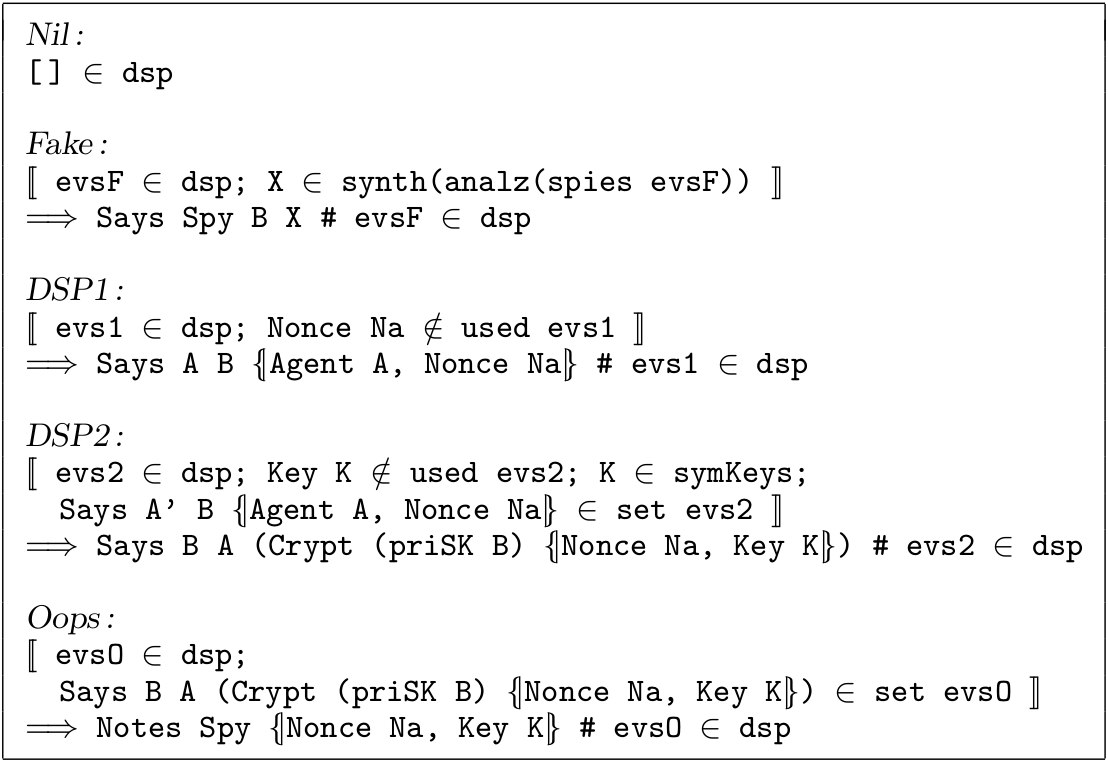
\includegraphics[width=0.8\textwidth]{img/prt-example-model}
  \label{fig:notation-example-model}
  \caption{Formal model for the protocol displayed in Figure \ref{prt:notation-example}. Figure is already following Isabelle's syntax}
\end{figure}

Two extra rules are defined. The first, \textit{Fake} relates to the spy ability to send any message that she can fake, i.e., any message $X \in \texttt{synth(analz(spies }\textit{evs} \texttt{))}$. Such rule is consistent with the Dolev-Yao attacker abstraction. The last rule, \textit{Oops}, abstracts the loss of a session key to the Spy, which is treated as a local security breach. This flaw may affect the whole system and this rule allows to detect such situations. Such rules may arise as a subgoal in the Isabelle system, needed to be manually stated, implying that the protocol has a natural flaw.

Using this model, a large gamma of traces can be constructed, although not every conceivable trace can be derived from it, since the model should impose some restrictions to the traces. Also, any desired protocol property should be verified against each model rule, a process which Isabelle helps to automatize. Thus, we defined that any property of the model is an attempt to formalize a protocol goal.


\section{Goals Verification}
Having a consistent model of the protocol is the first step to its full verification. Thus, it is necessary to identify the model properties and correlate them with its goals. Since it is an inductive method, a given property must be checked against all system points, including its rules. The formalization and latter verification of the goals innate to the protocol are the last part of the Inductive Method.

\subsection{Reliability}
Reliability relates to how close a model is to the system it is representing. Note that such crucial property may not be really related to the security protocol goals but to system goals itself. As a result, the number of reliability theorems may vary from a protocol to another.

However, some basic properties, which are common for many protocols, are already defined and likely to be used in new formalizations. Some of them may seem obvious, but are important for formal systems. As examples, we can cite the idempotence of \texttt{analz} operator, fresh keys and session keys proper distinction, and the certainty of messages composition correctness.

The theorems of this class are easy to proof. Many of these proofs are aided by Isabelle's simplifiers, which can easily reason about an given property inductively.

\subsection{Regularity}
The regularity lemmas are facts that can be proved from any message that appears in the traffic. Such properties may be applied to specific protocol goals, but some other broader properties can be guaranteed using them.

For example, regularity lemmas hold for long-term keys (or private keys), which can never be sent through the channel, since they are never meant to be used over the network, just in a agent local context. Therefore, it is easy to derive rules such:

\begin{center}
  Key(priK A) $\in$ parts(spies \textit{evs}) $\leftrightarrow$ $A \in bad$ \\
  Key(priK A) $\in$ analz(spies \textit{evs}) $\leftrightarrow$ $A \in bad$
\end{center}

\subsection{Confidentiality}
Holding confidentiality in a protocol can be simply translated as to preventing the disclosure of certain message to the Spy, that is, a message $X$ cannot belong the Spy knowledge set. Since messages are usually protected by encryption, this property is highly related to the use of keys. Precisely, the confidentiality of session keys is a major issue for the protocol confidentiality, because if a spy obtain a given session key, all messages encrypted with it could be easily altered by her. If we define a session key $K_{AB}$, we have to be certain that at the end of all traces the key does not belong to the knowledge set of the Spy. That said, we have the following:

\begin{center}
  Key $K_{AB} \notin$ analz(spies \textit{evs})
\end{center}

Note that, if key $K_{AB}$ is encrypted with some other private key of an agent, the latter cannot be part of the compromised agents set. Otherwise, the Spy could easily retrieve the key from the compromised agent, obtaining the session key and further messages.

Confidentiality is also interesting for nonces. Nonces are commonly used for computation of other protocol details, as keys and MACs \cite{bella-book}. Therefore, the model must provide confidentiality to all nonces used for composing important protocol pieces.


\subsection{Unicity}
The creation of fresh components in protocol is vastly used. It is seen in the production of keys, nonces and other entities and they are mostly used for a single session, identifying it. Therefore, providing freshness in a protocol resembles unicity, a concept that establishes bounds between a message and its fresh components.

More precisely, if two events contain the same fresh message component, then the events are identical. Further, events containing fresh message components cannot occur more than once, otherwise they violate the unicity concept.

A formalization for this definition prompted the creation of a new predicate in Isabelle/HOL \textit{Auth} library, the \texttt{Unique} predicate. It takes an event and a trace as parameters, holding if the given event is unique in the given trace. Such formalization is crucial for detecting replay attacks over traces.




\subsection{Authenticity}
This property can also be read as legitimacy. In the method, the guarantee of a message's authorship is presented as synonym of integrity, since if the message is unaltered (integrity), then the authorship must be preserved. Even if the Spy intercepts the message and them relays it to the recipient, if integrity is preserved, then legitimacy is still preserved, since the Spy acted as a channel relay.

As a result, it is important that the message's author does not belong to the compromised agent set. Conversely, any messages sent by him would be compromised as well and authenticity would not hold. Such concept may seem obvious for integrity matters, but it is important to enforce the authorship interest. Therefore, both properties are attached during our verifications.





\subsection{Authentication}
As discussed in Section \ref{sec:protocols:auth}, authentication may assume many properties. Supposing an initiator $A$, who completes a protocol session with a responder $B$. In this run, authentication may be translated as:

\begin{enumerate}
  \item \textbf{Aliveness of B}, meaning that $B$ has been running the protocol;
  \item \textbf{Weak agreement of $B$ with $A$}, meaning that $B$ has been running the protocol with $A$;
  \item \textbf{Non-injective agreement of $B$ with $A$ on $H$}, meaning a weak agreement of $B$ with $A$, considering the set $H$ of messages components;
  \item \textbf{Injective agreement of $B$ with $A$ on $H$}, meaning the non-injective agreement of $B$ with $A$, using the set $H$ of message components, where $B$ did not respond more than once on each session with $A$.
\end{enumerate}

The Inductive Method does not provide formalisms to reason about the fourth point. Although, it is claimed on \cite{bella-book} that such formalization can be easily constructed by simply verification of repetition of a given event \textit{ev} in the analyzed trace, restraining the agents to single responses. However, the method mainly tries to provide models that are more permissive as possible, stating that any message could be repeated over traces with no harm to model.

Specifically, non-injective agreements have a bigger focus. Regarding key distribution protocols, such property applied to session keys establishes a trust relation between the two agents, with a given key as a validation of such relationship, since both agents are uncompromised.

Eventually, \textbf{key distribution} becomes a major goal to be checked. Since this concept is related to the agreement of two agents in a mutual secret, it is stated in \cite{auth:bellare-rogaway} that this property is, indeed, stronger than authentication and thus, authentication itself relies on key distribution. Additionally, the authors of the Inductive Method proves that if authentication holds, so does key distribution, specifically non-injective agreement on a session key.
